
\documentclass[11pt]{article}
\usepackage{graphicx}
\usepackage{a4wide}
\usepackage[section]{placeins}
\begin{document}

\title{Steuerungsboard Doku}
\author{Lukas von Däniken}
\date{\today}
\maketitle
\newpage

\section{Bestückungsplan}
\begin{figure}[h]
	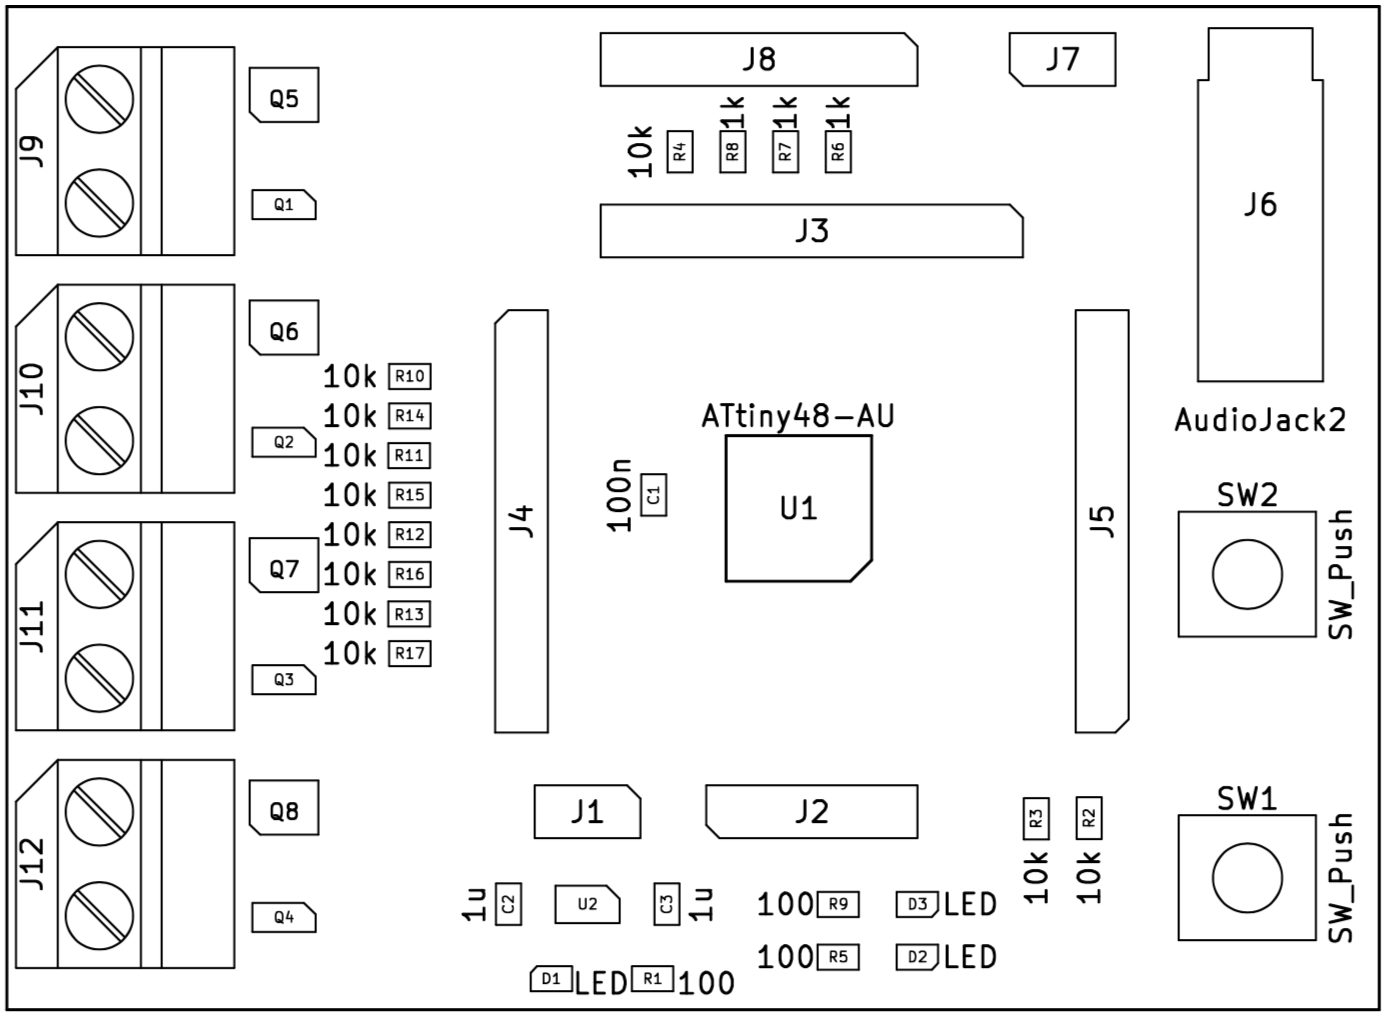
\includegraphics[width=1\textwidth]{graphics/Bestueckungsplan.png}
\end{figure}

\section{Pinbelegung}
\begin{minipage}[t]{0.3\textwidth}
	\begin{flushleft}
		\textbf{Stiftleiste J2}
	\end{flushleft}
	\begin{tabular}{l|l}
		Pin 1	&	PA0	\\\hline
		Pin 2	&	PA1	\\\hline
		Pin 3	&	PA2	\\\hline
		Pin 4	&	PA3	
	\end{tabular}
	\begin{flushleft}
		\textbf{Stiftleiste J5}
	\end{flushleft}
	\begin{tabular}{l|l}
		Pin 1	&	PD0	\\\hline
		Pin 2	&	PD1	\\\hline
		Pin 3	&	PD2	\\\hline
		Pin 4	&	PD3	\\\hline
		Pin 5	&	PD4	\\\hline
		Pin 6	&	PD5	\\\hline
		Pin 7	&	PD6	\\\hline
		Pin 8	&	PD7
	\end{tabular}
\end{minipage}
\begin{minipage}[t]{0.3\textwidth}
	\begin{flushleft}
		\textbf{Stiftleiste J3}
	\end{flushleft}
	\begin{tabular}{l|l}
		Pin 1	&	PB0\\\hline
		Pin 2	&	TX\\\hline
		Pin 3	&	RX\\\hline
		Pin 4	&	MOSI\\\hline
		Pin 5	&	MISO\\\hline
		Pin 6	&	SCK\\\hline
		Pin 7	&	FET1\\\hline
		Pin 8	&	FET2	
	\end{tabular}
	\begin{flushleft}
		\textbf{Stiftleiste J7}
	\end{flushleft}
	\begin{tabular}{l|l} 
 		Pin 1 & Rx \\ 
		\hline 
		Pin 2 & Tx \\ 
	\end{tabular} 
\end{minipage}
\begin{minipage}[t]{0.3\textwidth}
	\begin{flushleft}
		\textbf{Stiftleiste J4}
	\end{flushleft}
	\begin{tabular}{l|l}
		Pin 1	&	SW1\\\hline
		Pin 2	&	SW2\\\hline
		Pin 3	&  LED1	\\\hline
		Pin 4	&  LED2\\\hline
		Pin 5	&	FET3	\\\hline
		Pin 6	&	FET4	\\\hline
		Pin 7	&	RESET\\\hline
		Pin 8	&	PC7
	\end{tabular}
	\begin{flushleft}
		\textbf{Stiftleiste J8}
	\end{flushleft}
	\begin{tabular}{l|l}
		Pin 1	&	MOSI\\\hline
		Pin 2	&	MISO\\\hline
		Pin 3	&	SCK\\\hline
		Pin 4	&	RESET\\\hline
		Pin 5	&	3V3\\\hline
		Pin 6	&	GND
	\end{tabular}
\end{minipage}
\newpage

\section{Mikrocontroller flashen}
Damit die gewünschte Software auf den Mikrocontroller geladen werden kann müssen einige Vorbereitungen getroffen werden. Die Vorbereitungen lassen sich in die Teile Hardwaresetup und Softwaresetup aufteilen.
\subsection{Hardwaresetup}
Der Bereich Hardwaresetup zeigt auf, welche Vorbereitungen auf der physikalischen Schicht getroffen werden müssen, damit die kompilierte Software auf den Mikrocontroller geflashed werden kann.
Das Bild \ref{fig:flashSetup} zeigt, welche Verbindungen zwischen dem Steuerungsboard und dem Raspberrypi gebraucht werden. Dazu muss lediglich die Stiftleiste J8 verwendet werden, welche alle benötigten Pin's des Mikrocontrollers zu Verfügung stellt. Zudem sind die Widerstände bereits auf dem Steuerungsboard angebracht. Tabelle \ref{tab:flashConnects} zeigt die gebrauchten Verbindungen.

\begin{table}\label{tab:flashConnects}
	\begin{tabular}{l|l}
		J8-Pin1(MOSI)& GPIO10 \\\hline
		J8-Pin2(MISO)& GPIO09	\\\hline
		J8-Pin3(SCK)& GPIO11 \\\hline
		J8-Pin4(RESET)& GPIO12 \\\hline
		J8-Pin5(+3V3)& 3.3V \\\hline
		J8-Pin6(GND)& GND 
	\end{tabular}
\end{table}
\begin{figure}[h]\label{fig:flashSetup}
	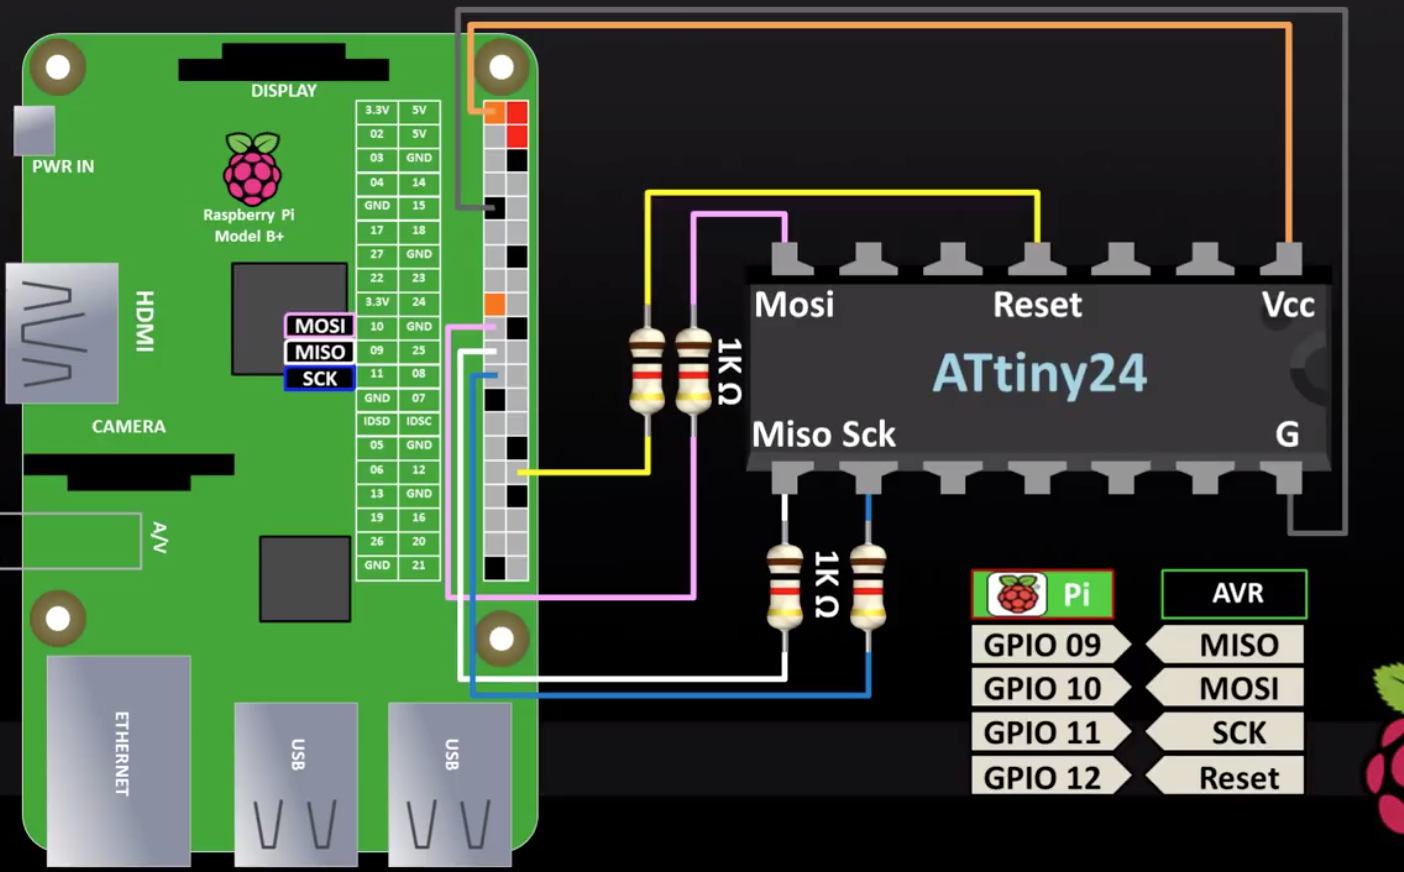
\includegraphics[width=1\textwidth]{graphics/flashen.png}
	\caption{Beschaltung Raspberrypi}
\end{figure}
\FloatBarrier
\subsection{Softwaresetup}

\end{document}


